\documentclass[10pt,a4paper]{article}

\usepackage[margin=0.5cm]{geometry}
\usepackage{multicol}
\usepackage{amsmath, amssymb}
\usepackage{tcolorbox}
\usepackage{enumitem}
\usepackage{makecell}
\usepackage{tabularx}
\usepackage{tikz}
\usepackage{pgfplots}
\pgfplotsset{compat=1.18} % latest stable

\usepackage{tikz}
\usepackage[utf8]{inputenc}
\usepackage[T1]{fontenc}
\usetikzlibrary{arrows.meta}

% compact lists
\setlist{nosep}

% compact sections
\setlength{\parindent}{0pt}
\setlength{\parskip}{0pt}

\begin{document}

\begin{center}
  \bfseries\Huge Questionario Socrative
\end{center}
\vspace{20pt}

1. En una celda IEEE 802.11b en modo infraestructura y MAC DCF, hay 14 dispositivos finales activos.
El tamaño de las tramas MAC de datos es de 98 B. ¿Cuánto vale el throughput medio disponible por estación?
La velocidad nominal es la máxima permitida por esta especificación de capa física.

\begin{enumerate}[label=\alph*]
    \item 85.2 Kbps aprox.
    \item \textbf{79.4 Kbps aprox.}
    \item 84.0 Kbps aprox.
    \item 90.0 Kbps aprox.
    \item Todas las respuestas restantes son falsas.
\end{enumerate}

\textbf{Explicación}

Ejecutando el código que implementa el método de Bianchi, para sta = 15 (las 14 estaciones juntamente con el
punto de acceso tienen que competir por el canal), y payload = 98-34 = 64 B (la sobrecarga de las tramas Wi-Fi
es de 34 B), se obtiene eficiencia = 0.108 aprox. El throughput medio por estación es, por tanto: 
$\frac{11\cdot0.108}{15} = 0.0794$ Mbps $= 79.4$ Kbps.

\vspace{15pt} \hrule \vspace{15pt}




2. Cuatro estaciones sondean un canal Ethernet sobre medio compartido y lo encuentran ocupado.
Suponiendo que todas van a experimentar la primera colisión, ¿cuál es la probabilidad de que una cualquiera de
ellas consiga transmitir con éxito en el primer intento?


\begin{enumerate}[label=\alph*]
    \item 0.25
    \item \textbf{0.50}
    \item 0.125
    \item 0.0625
    \item Todas las respuestas restantes son falsas.
\end{enumerate}

\textbf{Explicación}

La probabilidad de que una estación concreta transmita con éxito es la probabilidad de que dicha estación elija
un slot y las otras tres elijan el otro slot. Eso ocurre con probabilidad $2\cdot0.5\cdot0.5^3 = 2\cdot0.5^4$
(la multiplicación por 2 es para tener en cuenta que hay dos formas de conseguir la transmisión en el primer
intento, es decir, transmitir con éxito en el primer slot o transmitir con éxito en el segundo slot).
Puesto que la estación concreta puede ser, en realidad, cualquiera de las cuatro, hay 4 formas de que se cumpla
la condición anterior, por lo que el resultado definitivo es $4\cdot2\cdot0.5^4 = 0.5$.

\vspace{15pt} \hrule \vspace{15pt}




3. Señalar la afirmación correcta:

\begin{enumerate}[label=\alph*]
    \item Un dispositivo conectado a una celda Wi-Fi se desplaza y se engancha a una celda Wi-Fi con un SSID distinto. Se trata de una re-asociación.
    \item Un dispositivo recibe una trama Ethernet y la detecta errónea. Entonces, solicita la retransmisión de dicha trama.
    \item En un mismo dispositivo, la dirección Ethernet y la dirección Wi-Fi coinciden.
    \item Un usuario activa la zona Wi-Fi de su teléfono móvil. Significa que va a utilizar Wi-Fi Direct.
    \item \textbf{En las redes Wi-Fi, el mecanismo de control de errores es del tipo stop-and-wait ARQ.}
\end{enumerate}

\textbf{Explicación}

Si el SSID cambia, es que el dispositivo cambia de red Wi-Fi, y por tanto no se trata de una re-asociación, sino de una asociación a una nueva red Wi-Fi (deberá iniciarse una nueva autenticación).

Cuando un dispositivo recibe una trama Ethernet y la detecta errónea, la descarta sin solicitar su retransmisión.

Las direcciones Ethernet y Wi-Fi de un mismo dispositivo son distintas.

Efectivamente, el mecanismo de control de errores en las redes Wi-Fi es del tipo stop-and-wait ARQ, puesto que por cada trama de datos enviada por una estación, ésta espera recibir un ACK, y si no lo recibe retransmite la trama.

Cuando un usuario activa la zona Wi-Fi de su teléfono móvil, lo está convirtiendo en un punto de acceso.

\vspace{15pt} \hrule \vspace{15pt}




4.  Señalar cuál de las siguientes afirmaciones acerca de las redes Ethernet es correcta:

\begin{enumerate}[label=\alph*]
    \item En Ethernet sobre medio compartido, las colisiones se detectan por la no recepción de un ACK.
    \item \textbf{En Ethernet sobre medio compartido, las tramas colisionadas se retransmiten, y las no colisionadas, pero detectadas erróneas, se descartan.}
    \item En Ethernet conmutado, las tramas erróneas se reenvían siempre.
    \item En Ethernet sobre medio compartido y topología en estrella o árbol centrada en hub, el hub sólo repite las tramas que recibe correctamente.
    \item En Ethernet conmutado, las transmisiones son half-duplex.
\end{enumerate}

\textbf{Explicación}
En Ethernet, sólo hay retransmisión de tramas cuando es sobre medio compartido y se produce colisión de tramas. En el resto de casos, las tramas se descartan sin retransmisión.

Un hub repite la trama que recibe por un puerto de entrada por los restantes puertos de salida, sea correcta o no, pues este dispositivo no analiza el contenido de la misma.

En Ethernet conmutado, cada dispositivo final tiene un enlace punto a punto bidireccional y full-duplex con un conmutador.

\vspace{15pt} \hrule \vspace{15pt}




5.  Señalar cuál de las siguientes afirmaciones acerca de las redes Wi-Fi es correcta:

\begin{enumerate}[label=\alph*]
    \item El acceso RTS-CTS permite eliminar el problema del terminal expuesto.
    \item Todas las estaciones de una misma celda se ven entre sí.
    \item \textbf{Una estación avanza una etapa en el algoritmo de backoff cada vez que deja de recibir el ACK de una trama.}
    \item Una estación activa el algoritmo de backoff para una trama a partir de la primera vez que dicha trama colisiona.
    \item Implementan el mecanismo CSMA/CD.
\end{enumerate}

\textbf{Explicación}
El acceso RTS-CTS sirve para solucionar el problema del terminal escondido.

En una celda Wi-Fi, no es necesario que las estaciones tengan que verse directamente.

Efectivamente, una estación avanza una etapa en el algoritmo de backoff cada vez que deja de recibir el ACK de una trama. Este algoritmo se activa con la detección del canal ocupado, no con la primera colisión.

El mecanismo CSMA/CD es el de las redes Ethernet, y no es viable en redes Wi-Fi.

\vspace{15pt} \hrule \vspace{15pt}




6.  Señalar cuál de las siguientes afirmaciones acerca de las redes Wi-Fi es correcta:


\begin{enumerate}[label=\alph*]
    \item Las comunicaciones son full-duplex.
    \item El acceso RTS-CTS sólo es recomendable para tramas cortas.
    \item Las colisiones siempre se deben a terminales escondidos.
    \item PCF implica que hay punto de acceso y DCF implica que no lo hay.
    \item \textbf{Wi-Fi Direct es un caso especial de red Wi-Fi en modo ad-hoc.}
\end{enumerate}

\textbf{Explicación}

En las redes Wi-Fi con mecanismo DCF, el medio es compartido y no es posible la comunicación full-duplex. Si el mecanismo es PCF tampoco, pues cuando le toca el turno a una estación, puede ser para transmitir o recibir, pero no las dos cosas a la vez.

El acceso RTS-CTS es especialmente no recomendable para el envío de tramas cortas, pues es cuando resulta más ineficiente.

Muchas colisiones tienen lugar entre estaciones que ejecutan el algoritmo de backoff, independientemente de que se vean o no.

El mecanismo DCF opera tanto en el modo infraestructura como en el modo ad-hoc (en este último es donde falta el punto de acceso).

Wi-Fi Direct es un caso especial de red Wi-Fi en modo ad-hoc, pues no utiliza ningún tipo de infraestructura de apoyo.

\vspace{15pt} \hrule \vspace{15pt}





\begin{multicols}{2}
    7.  La figura representa la red de una organización, sin mostrar la conexión a la Internet pública. El bloque asignado por el ISP es 192.168.5.128/25. El administrador aplica subnetting bajo el criterio de bloques contiguos, orden decreciente del tamaño de las subredes IP y orden creciente de las direcciones IP. ¿Qué bloque habrá asignado a la LAN A, si esta subred interconecta 13 dispositivos finales?
    
    \begin{enumerate}[label=\alph*]
        \item \textbf{192.168.5.224/28}
        \item 192.168.5.240/28
        \item 192.168.5.196/27
        \item 192.168.5.160/28
        \item 192.168.5.224/27
    \end{enumerate}
    \columnbreak
    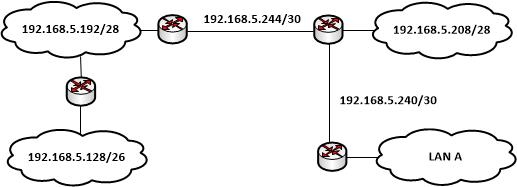
\includegraphics[width=0.5\textwidth]{1.jpeg}
\end{multicols}

\textbf{Explicación}

El bloque asignado a la LAN A tiene que tener un tamaño de 13 + 1 + 2 = 16, y por tanto necesita 4 bits libres, lo que implica un prefijo /28. El siguiente bloque a  192.168.5.208/28 es 192.168.5.224/28.

\vspace{15pt} \hrule \vspace{15pt}




8.  Un computador conectado a una red Ethernet ejecuta una aplicación que hace uso del protocolo de transporte TCP. Suponiendo que el direccionamiento es IPv6, ¿cuánto vale el parámetro MSS de la conexión?

\begin{enumerate}[label=\alph*]
    \item 1460 B.
    \item 1452 B.
    \item \textbf{1440 B.}
    \item 1472 B.
    \item 1466 B.
\end{enumerate}

\textbf{Explicación}

El valor MTU de Ethernet es 1500 B. Si le restamos los 40 B de cabecera IPv6 y los 20 B de cabecera TCP, resulta un valor de MSS de 1440 B.

\vspace{15pt} \hrule \vspace{15pt}




9.  Cinco estaciones Wi-Fi (A, B, C, D y E) están alineadas, de forma que cada estación solamente se ve con sus vecinas inmediatas. Supongamos que inicialmente el canal está inactivo y, a continuación, se producen los siguientes acontecimientos en el orden temporal indicado:

\begin{enumerate}
    \item D transmite a E.
    \item C quiere transmitir a B.
    \item A quiere transmitir a B.
\end{enumerate}

Para esta secuencia de acontecimientos, señalar cuál de las siguientes afirmaciones refleja la situación producida:

\begin{enumerate}[label=\alph*]
    \item Se produce una colisión en la estación B.
    \item C transmite con éxito a B y D transmite con éxito a E.
    \item \textbf{A transmite con éxito a B y D transmite con éxito a E.}
    \item Sólo tiene lugar la transmisión de D a E.
    \item Se produce una colisión en la estación E.
\end{enumerate}

\textbf{Explicación}

D transmite con éxito a E y C se abstiene de transmitir a B por estar expuesto a la transmisión de D. A no detecta ninguna señal en el medio y transmite con éxito a B, sin que se produzca colisión en B porque C decidió no transmitir.

\vspace{15pt} \hrule \vspace{15pt}




10.  El protocolo ARP se puede usar en combinación con el protocolo DHCP para la detección de direcciones duplicadas (DAD). Consiste en que cuando un servidor DHCP ofrece una dirección IP a un dispositivo a través del mensaje DHCP offer, el dispositivo envía un ARP request sobre esa misma dirección IP ofrecida, de manera que si obtiene respuesta, es que dicha dirección ya ha sido asignada a otro dispositivo en la misma red. ¿Cuáles son los valores de los parámetros SHA, SPA y TPA del mensaje ARP request?


\begin{enumerate}[label=\alph*]
    \item SHA: @MAC dispositivo \\
    SPA: @IP dispositivo \\
    TPA: @IP ofrecida \\
    
    \item \textbf{SHA: @MAC dispositivo \\
    SPA: 0.0.0.0 \\
    TPA: @IP ofrecida} \\
    
    \item SHA: @MAC dispositivo \\
    SPA: @IP dispositivo \\
    TPA: @IP servidor DHCP \\
    
    \item SHA: @MAC servidor DHCP \\
    SPA: 0.0.0.0 \\
    TPA: @IP ofrecida \\
    
    \item SHA: FF:FF:FF:FF:FF:FF \\
    SPA: 0.0.0.0 \\
    TPA: 255.255.255.255 \\
\end{enumerate}

\textbf{Explicación}

Hay que tener en cuenta que el dispositivo que ejecuta el DAD todavía carece de dirección IP, por lo que tiene que utilizar la dirección IP 0.0.0.0 como valor SPA, la cual indica precisamente dirección IP no asignada. El valor SHA será su dirección física (dirección MAC) y, lógicamente, deberá ejecutar el DAD sobre la IP que se le ha ofrecido si quiere averiguar si otro dispositivo ya la tiene (error que podría ser causado por el servidor DHCP, por ejemplo, por culpa de una mala configuración).

\vspace{15pt} \hrule \vspace{15pt}




11.  Señalar cuál de las siguientes afirmaciones es correcta:

\begin{enumerate}[label=\alph*]
    \item Una aplicación se ejecuta sobre el protocolo UDP. El contenido del campo Protocol de los datagramas IPv4 es 00000110.
    \item El ensamblado de datagramas IPv4 fragmentados puede realizarse tanto en un router intermedio como en un dispositivo final.
    \item RIP es un protocolo de aplicación, ya que se ejecuta sobre el protocolo de transporte UDP.
    \item \textbf{En una conexión TCP, el valor MSS es 1460 B. Suponiendo que se envía un segmento de tamaño máximo, el valor hexadecimal del campo Total Length de un datagrama IPv4 estándar que lo encapsule es 05DC.}
    \item Todas las restantes respuestas son falsas.
\end{enumerate}

\textbf{Explicación}

Cuando el protocolo de transporte es UDP, el campo Protocol de los datagramas es 17 en decimal, que no corresponde a la secuencia binaria dada.

Los datagramas IP fragmentados sólo pueden ensamblarse en el dispositivo final.

RIP se ejecuta sobre UDP, pero es un protocolo del plano de control que nada tiene que ver con los protocolos de aplicación.

Si MSS = 1460, entonces el tamaño de los datagramas es 1460 + 20 + 20 = 1500 B (las cabeceras TCP e IP tienen un tamaño de 20 B cada una), y ese es el valor que va a tener el tamaño total del datagrama estándar, es decir, sin incluir opciones. El valor 1500 en hexadecimal es 05DC.

\vspace{15pt} \hrule \vspace{15pt}




12.  Señalar cuál de las siguientes afirmaciones es correcta:

\begin{enumerate}[label=\alph*]
    \item En un conmutador Ethernet, se desencapsula el paquete de una trama, se examina su dirección IP de destino, y se determina el puerto de salida.
    \item \textbf{Un ordenador portátil se desengancha de un punto de acceso y se engancha a otro punto de acceso de la misma subred IP. Ni su dirección IP ni su dirección física habrán cambiado.}
    \item En una red Metro Ethernet, el encaminamiento se realiza en base a direcciones IP.
    \item Las diversas jerarquías digitales (E-carrier, T-carrier, etc.) son especificaciones de capa de enlace OSI.
    \item Las líneas serie sólo permiten cubrir conexiones sobre distancias cortas.
\end{enumerate}

\textbf{Explicación}

El conmutador Ethernet decide en base a direcciones físicas, no direcciones IP.

En efecto, si un portátil se mantiene dentro de la misma subred IP aunque cambie de punto de acceso, su dirección IP no cambia, y evidentemente su dirección física tampoco.

Una red Metro Ethernet es básicamente una red Ethernet conmutada de largo alcance, y ejecuta el encaminamiento en base a direcciones físicas.

Las jerarquías digitales son soluciones de la capa física de OSI.

Las líneas serie son soluciones WAN punto a punto.

\vspace{15pt} \hrule \vspace{15pt}




13.  ¿Cuánto vale la velocidad media disponible por estación en una red Ethernet 1000BASE-T que interconecta 20 estaciones, todas activas? Suponer tramas de tamaño máximo.


\begin{enumerate}[label=\alph*]
    \item \textbf{26.5 Mbps aprox.}
    \item 529.3 Mbps aprox.
    \item 45 Mbps aprox.
    \item 21.5 Mbps aprox.
    \item 6.2 Mbps aprox.
\end{enumerate}

\textbf{Explicación}

Ethernet 1000BASE-T es sobre medio compartido. Se trata de aplicar la fórmula de eficiencia con $N = 20$ estaciones
y $\tau_b = 4096$ bits (duración equivalente en bits de los slots de contención).
Al multiplicar la eficiencia resultante por la velocidad nominal (1000 Mbps) y dividir por el total de
estaciones, se obtienen 26.5 Mbps aprox. por estación.

\vspace{15pt} \hrule \vspace{15pt}




\begin{multicols}{2}
    14. ¿Cuántos dominios de colisión (C) y dominios de broadcast (B) hay en la red de la figura?

    \begin{enumerate}[label=\alph*]
        \item C = 5, B = 1.
        \item C = 4, B = 3.
        \item C = 4, B = 1.
        \item \textbf{C = 5, B = 3.}
        \item Todas las respuestas restantes son falsas.
    \end{enumerate}
    \columnbreak
    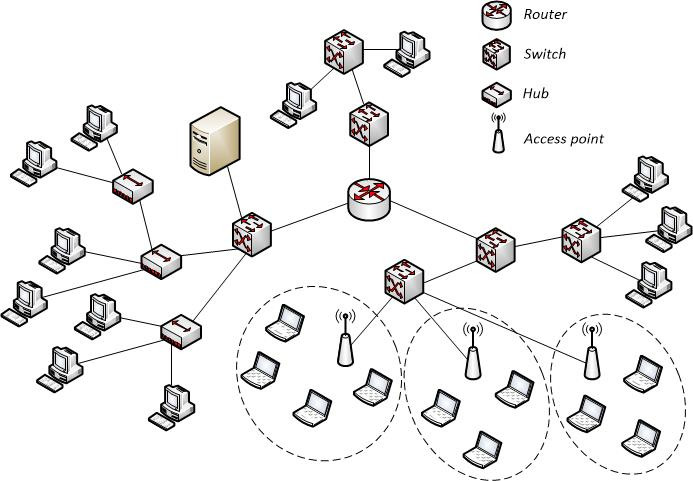
\includegraphics[width=0.5\textwidth]{2.jpeg}
\end{multicols}

\textbf{Explicación}

Hay 2 topologías Ethernet sobre medio compartido independientes, y 3 celdas Wi-Fi, lo que da un total de 5 dominios de colisión. Los dominios de broadcast coinciden siempre con las subredes IP, por lo que en total hay 3.

\vspace{15pt} \hrule \vspace{15pt}





15. ¿Cuál es el valor binario del campo IHL de la cabecera de un datagrama IPv4?


\begin{enumerate}[label=\alph*]
    \item \textbf{0101.}
    \item 0110.
    \item 1111.
    \item 0100.
    \item 00000101.
\end{enumerate}

\textbf{Explicación}

El campo IHL tiene un longitud de 4 bits y expresa el tamaño total de la cabecera IPv4 en palabras de 32 bits. La cabecera IPv4 estándar tiene un tamaño de 20 B, lo que equivale a 5 palabras de 32 bits. El valor decimal 5 es 0101 en binario.

\vspace{15pt} \hrule \vspace{15pt}




16.  En una red Ethernet sobre medio compartido, 4 estaciones sondean el canal y lo encuentran ocupado. Tras el primer slot de colisión inevitable, las 4 estaciones activan el algoritmo BEB con 2 slots (primera etapa). ¿Cuál es la probabilidad de que las 4 estaciones tengan que ejecutar la segunda etapa del algoritmo?

\begin{enumerate}[label=\alph*]
    \item 0.125.
    \item 0.375.
    \item 0.4375.
    \item 0.3125.
    \item 0.5
\end{enumerate}

\textbf{Explicación}

La única forma de que se produzca una transmisión con éxito en la primera etapa es que una de las estaciones
elija un slot y las restantes elijan el otro slot. Si les damos nombre a las estaciones, por ejemplo,
A, B, C y D, y suponemos que es la estación A que transmite con éxito, la probabilidad de que eso ocurra es
$2\cdot0.5\cdot0.5^3$ (el 2 proviene de que A puede transmitir con éxito en el primer slot o en el segundo,
por lo que hay 2 opciones). Como no tiene por qué ser A la que transmita con éxito, sino que puede ser
cualquiera de las 4 estaciones, multiplicamos el resultado anterior por 4: $4\cdot2\cdot0.5\cdot0.5^3 = 0.5$.
La probabilidad solicitada es la complementaria de este valor, es decir, 0.5.

\vspace{15pt} \hrule \vspace{15pt}




\begin{multicols}{2}
    17. CG-NAT (Carrier Grade - NAT) es una extensión de NAT con sobrecarga a mayor escala, como es el ámbito de los ISP locales. En este caso, el conjunto de direcciones privadas es 100.64.0.0/10 (RFC 6598). La figura adjunta muestra un escenario de aplicación. Determinar cuál de las siguientes afirmaciones es correcta. 

    \begin{enumerate}[label=\alph*]
        \item La administración de direcciones IPv4 podría reducirse al consumo de una sola dirección IPv4 pública, que quedaría asignada a la interfaz del router R con el ISP local.
        \item La administración de direcciones IPv4 podría reducirse al consumo de tantas direcciones IPv4 públicas como routers POP, las cuales quedarían asignadas a las interfaces de tales routers con la red núcleo del ISP local.
        \item \textbf{La administración de direcciones IPv4 podría reducirse al consumo de una sola dirección IPv4 pública, que quedaría asignada a la interfaz del router R con el ISP de nivel 2.}
        \item La administración de direcciones IPv4 podría reducirse al consumo de tantas direcciones IPv4 públicas como routers POP, las cuales quedarían asignadas a las interfaces de tales routers con las redes de usuario.
        \item Supongamos que un usuario solicita desactivar el servicio CG-NAT a su ISP. Entonces, el usuario consumiría una IPv4 pública que quedaría asignada a la interfaz entre la red del usuario y el router POP correspondiente.
    \end{enumerate}
    \columnbreak
    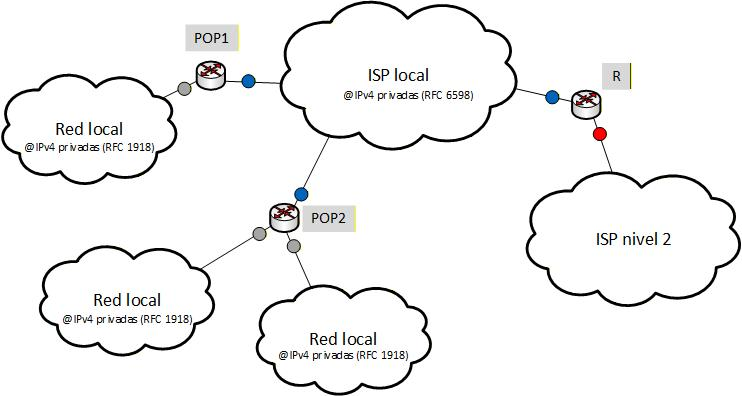
\includegraphics[width=0.5\textwidth]{3.jpeg}
\end{multicols}

\textbf{Explicación}

El servicio habitual de NAT con sobrecarga implica que la red local (red de usuario) consume una sola dirección IPv4 pública, que queda asignada a la interfaz del router puerta de enlace con el router POP. El servicio CG-NAT consiste en extender el ahorro de direcciones IPv4 públicas de manera que todo el ISP local consume una sola dirección IPv4 pública, la cual queda asignada a la interfaz del router R con el siguiente ISP (por ejemplo, de nivel 2). El router R sería el encargado de hacer la traducción CG-NAT (router CG-NAT). El criterio es que las direcciones IPv4 públicas siempre se asignan de puertas hacia fuera. Resumiendo:

- Las interfaces marcadas con un punto gris, tendrían asignadas una dirección IPv4 privada de cualquiera de los bloques incluidos en el RFC 1918.

- Las interfaces marcadas con un punto azul, tendrían asignadas una 

 dirección IPv4 privada del bloque considerado en el RFC 6598.

- La interfaz marcada con un punto rojo tendría asignada una dirección IPv4 pública.

De este modo, con solo una IPv4 pública se administrarían todas las interfaces del ámbito del ISP local, en lugar de consumir una IPv4 pública por cada red de usuario. Téngase en cuenta que, al igual que ocurre con el servicio NAT convencional, las direcciones IPv4 del servicio CG-NAT no son enrutables fuera del ISP local, lo que significa que son reutilizables de un ISP local a otro.

\vspace{15pt} \hrule \vspace{15pt}




18.  Considérese la siguiente especificación para un bloque de direcciones IPv4: 172.215.17.0/25. Señalar cuál de las siguientes afirmaciones es correcta:


\begin{enumerate}[label=\alph*]
    \item El administrador de red puede configurar hasta 128 direcciones IPv4 individuales.
    \item \textbf{La dirección de broadcast es 172.215.17.127.}
    \item Es una especificación de bloque incorrecta.
    \item La dirección de broadcast es 172.215.17.255.
    \item La dirección 172.215.17.130 está incluida en el bloque.
\end{enumerate}

\textbf{Explicación}

Si el bloque de direcciones tiene un prefijo de longitud 25, significa que hay 7 bits para el identificador de host. Con 7 bits, hay 128 combinaciones posibles, pero hay 2 reservadas que no pueden ser utilizadas para direcciones IP individuales.

La dirección de broadcast se obtiene al fijar a 1 toda la parte libre, que en este caso son los últimos 7 bits. El último octeto queda así: 01111111, lo que corresponde al valor 127.

La dirección 172.215.17.130 está por encima de la dirección IP más alta dentro del bloque, que es la dirección de broadcast, por lo que queda fuera del mismo.

\vspace{15pt} \hrule \vspace{15pt}




19.  ¿Qué tipo de dirección es 255.255.255.255?


\begin{enumerate}[label=\alph*]
    \item Una dirección de broadcast Ethernet o Wi-Fi.
    \item Un broadcast dirigido a nivel IP.
    \item Una dirección unicast a nivel IP.
    \item \textbf{Un broadcast limitado a nivel IP.}
    \item Puede ser el contenido del campo de dirección origen de un paquete IP.
\end{enumerate}

\textbf{Explicación}

Se trata de una dirección IP (IPv4) que corresponde a lo que se conoce como broadcast limitado, porque los destinatarios son todos los dispositivos de la misma subred IP. Es limitado porque se circunscribe a la misma red local, pues un paquete con esta dirección como dirección de destino puede cruzar un router. Las direcciones multicast o broadcast nunca pueden funcionar como dirección origen.

\vspace{15pt} \hrule \vspace{15pt}




20.  En un canal Wi-Fi que opera según el mecanismo DCF, ¿qué tiempo mínimo transcurre entre el final de una trama transmitida con éxito y el comienzo de la siguiente? (Se entiende que ACK es la duración de los acuses de recibo y DATA la duración de las tramas de datos).

\begin{enumerate}[label=\alph*]
    \item DIFS.
    \item DATA + SIFS + ACK + DIFS.
    \item \textbf{SIFS + ACK + DIFS.}
    \item SIFS + ACK + SIFS.
    \item DATA + ACK + DIFS.
\end{enumerate}

\textbf{Explicación}

Entre el final de una trama transmitida con éxito y el comienzo de la siguiente debe transcurrir un tiempo mínimo de SIFS + ACK + DIFS. El valor SIFS es la separación entre el final de la trama de datos y el comienzo del acuse de recibo, y DIFS es el tiempo que debe transcurrir desde que el canal vuelve al estado inactivo (cuando termina la transmisión del acuse de recibo) hasta que una estación pueda transmitir una nueva trama.

\vspace{15pt} \hrule \vspace{15pt}




21.  Un router recibe un datagrama IPv4 cuyo tamaño total es de 3520 B, que debe reenviar a través de una red Ethernet (no se admiten tramas Jumbo). Suponiendo que genera el máximo número de tramas con el máximo tamaño que sea posible en el proceso de fragmentación, indicar cuál de las siguientes afirmaciones es correcta:

\begin{enumerate}[label=\alph*]
    \item Se generan tres datagramas, dos de tamaño 1520 B, y un tercero de tamaño 520 B.
    \item \textbf{Se generan tres datagramas con valores de Fragment Offset sucesivos iguales a 0, 185 y 370.}
    \item Se generan tres datagramas con valores de Fragment Offset sucesivos iguales a 0, 148 y 296.
    \item Se generan cuatro datagramas con valores de Fragment Offset sucesivos iguales a 0, 125, 250 y 375.
    \item Se generan cuatro datagramas con valores de Fragment Offset sucesivos iguales a 0, 110, 220 y 330.
\end{enumerate}

\textbf{Explicación}

Si se ha de generar el máximo número de tramas Ethernet con el tamaño máximo posible después de la fragmentación, quiere decir que el campo de datos de los fragmentos deberá tener un tamaño de 1480 B, puesto que éste es el máximo múltiplo de 8 que, sumado luego con el tamaño de la cabecera IPv4, da el máximo campo de datos de las tramas Ethernet (MTU de Ethernet es 1500 B). Si el datagrama recibido tiene un tamaño de 3520 B, al restarle la cabecera resulta un campo de datos de 3500 B, que da lugar a 2 campos de datos de 1480 B y un tercer campo de datos de 540 B. Puesto que 1480/8 es 185, los valores sucesivos de Fragment Offset de los 3 datagramas resultantes de la fragmentación son 0, 185 y 370.

\vspace{15pt} \hrule \vspace{15pt}




22.  Señalar cuál de las siguientes afirmaciones es correcta:

\begin{enumerate}[label=\alph*]
    \item El tamaño máximo de una cabecera IPv4 es 20 B.
    \item Siempre, todos los datagramas IPv4 de una misma conexión se encaminan a través de la misma ruta.
    \item \textbf{Cada vez que un router reenvía un datagrama IPv4, recalcula el valor del campo Header Checksum de la cabecera del mismo.}
    \item La dirección IPv4 origen de un datagrama va cambiando a medida que dicho datagrama salta de una red a otra en su camino al destinatario.
    \item Los segmentos TCP de la fase de establecimiento de una conexión previa a una descarga web forman parte del plano de control.
\end{enumerate}

\textbf{Explicación}

El tamaño estándar de una cabecera IPv4 es 20 B, pero su tamaño máximo es 60 B.

Puesto que IP no ofrece un servicio orientado a la conexión que busque una ruta antes de que la transferencia de datos tenga lugar, no está garantizado que los datagramas de una misma conexión se encaminen por la misma ruta.

En efecto, la comprobación de errores tiene que recalcularse cada vez que un router reenvía un datagrama, puesto que, como mínimo, el campo TTL del mismo habrá cambiado.

En el transcurso de una conexión Internet, las direcciones IP origen y destino de cada datagrama se mantienen fijas.

Los segmentos TCP de la fase de establecimiento de una conexión son segmentos de control, pero forman parte del plano de datos si proceden de la ejecución de una aplicación de usuario, como es el caso de la descarga de una página web.

\vspace{15pt} \hrule \vspace{15pt}




\begin{multicols}{2}
    23. El siguiente escenario muestra un servidor y un servidor redundante o de reserva conectados a una red Ethernet conmutada. En un momento dado, el servidor redundante pasa a estar operativo en substitución del servidor habitual. ¿Qué mensaje podría utilizar el nuevo servidor para anunciarse?

    \begin{enumerate}[label=\alph*]
        \item Un mensaje DHCP offer.
        \item Un mensaje ICMP redirect for host.
        \item Un mensaje ICMP echo reply.
        \item \textbf{Un mensaje GARP.}
        \item Las otras respuestas son falsas.
    \end{enumerate}
    \columnbreak
    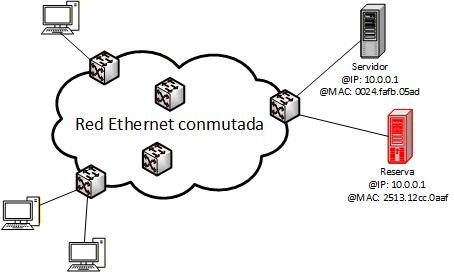
\includegraphics[width=0.5\textwidth]{4.jpeg}
\end{multicols}

\textbf{Explicación}

En realidad, lo único que tiene que anunciar el servidor redundante es el nuevo emparejamiento entre dirección IP y dirección MAC. Ello se consigue con un solo mensaje GARP, evitando así que la red se sobrecargue posteriormente con mensajes ARP request generado por los dispositivos que quieren acceder a dicho servidor.

\vspace{15pt} \hrule \vspace{15pt}




24.  ¿Cuál de las siguientes afirmaciones es correcta?

\begin{enumerate}[label=\alph*]
    \item Un router recibe un paquete cuya dirección IP de destino corresponde a una de sus subredes IP, pero ningún host de esa subred tiene dicha dirección IP. El router enviará un mensaje ICMP con campo Type = 3 y campo Code = 6.
    \item En una red Ethernet, el módulo ARP de un cierto dispositivo conectado a ella recibe un mensaje ARP response. Ese módulo ARP averigua la dirección local del dispositivo buscado gracias a que dicha dirección aparece como dirección origen de la trama Ethernet que encapsula el  ARP response recibido.
    \item En Internet, la ruta de ida y la ruta de vuelta entre dos dispositivos coinciden.
    \item En Internet, todos los paquetes que van en un mismo sentido de la comunicación, siguen la misma ruta siempre.
    \item Si al ejecutar un comando ping no se recibe respuesta, puede ser porque en la red del destinatario existe un cortafuegos que lo bloquea.
\end{enumerate}

\textbf{Explicación}

El router devolvería un mensaje ICMP con campo Type = 3 y campo Code = 7.

El módulo ARP averiguaría la dirección Ethernet del dispositivo buscado porque dicha dirección aparecería en el contenido del campo de datos del mensaje ARP response, no porque dicha dirección aparece como campo de dirección origen en la trama Ethernet que lo encapsula. El módulo ARP nunca llega a ver ese campo, ya que le llega el contenido desencapsulado de dicha trama.

En Internet, los paquetes de una conexión no tienen por qué ir por el mismo camino, independientemente de si van en un sentido o en otro.

Efectivamente, el administrador de una red puede bloquear los mensajes ICMP echo request.


\vspace{15pt} \hrule \vspace{15pt}




25.  Sobre la fragmentación de paquetes IPv4, ¿cuál de las siguientes afirmaciones es verdadera?


\begin{enumerate}[label=\alph*]
    \item La realiza el módulo TCP del host origen.
    \item \textbf{La realiza un router cuando lo requiere la MTU de la red del siguiente salto.}
    \item El ensamblado de los paquetes fragmentados lo ejecuta el módulo TCP del host de destino.
    \item A lo sumo, sólo puede haber una fragmentación a lo largo de una ruta.
    \item Las otras respuestas son falsas.
\end{enumerate}

\textbf{Explicación}

La fragmentación a nivel IP la realiza un router cuando el siguiente salto es una red con un valor MTU más restrictivo (no confundir con la segmentación que ejecuta el protocolo TCP). Puede realizarse tantas veces como sea necesario a lo largo de una ruta, pero cualquier paquete resultante de un proceso de fragmentación mantiene un vínculo con el paquete del cual procede (esto puede extenderse a varias "generaciones"). De este modo, se pueden ensamblar todos los fragmentos de forma correcta, las veces que sea necesario hasta reconstituir los paquetes originalmente enviados por la fuente. Los routers nunca ensamblan; es el módulo IPv4 del host de destino el que realiza el ensamblado antes de desencapsular el segmento y entregarlo al módulo de transporte superior.

\vspace{15pt} \hrule \vspace{15pt}

\end{document}